\documentclass[tikz,border=10pt]{standalone}
\usepackage{tikz}
\usetikzlibrary{shapes.geometric, arrows, positioning, fit, shadows, patterns}

\begin{document}

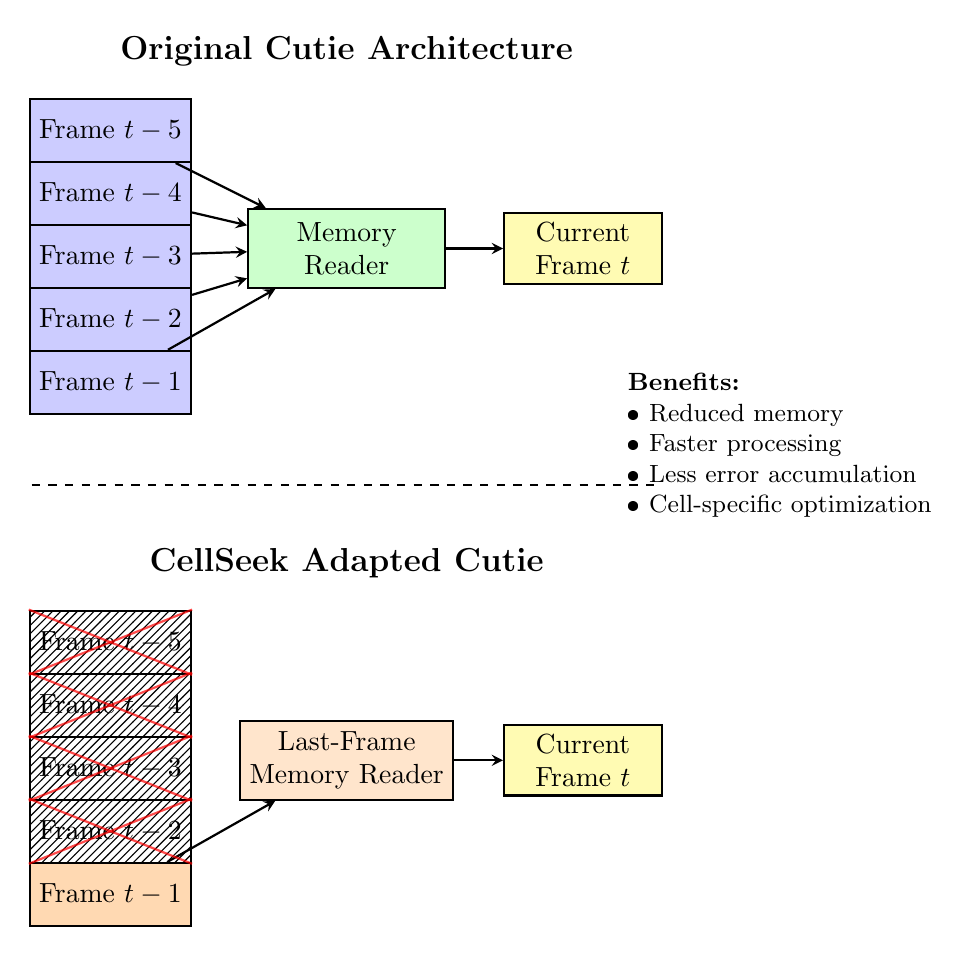
\begin{tikzpicture}[
    memory/.style={rectangle, draw, thick, fill=blue!20, minimum width=2cm, minimum height=0.8cm, align=center},
    memory_light/.style={rectangle, draw, thick, fill=blue!10, minimum width=2cm, minimum height=0.8cm, align=center},
    processor/.style={rectangle, draw, thick, fill=green!20, minimum width=2.5cm, minimum height=1cm, align=center},
    arrow/.style={->, >=stealth, thick},
    title/.style={font=\large\bfseries}
  ]

  % Original Cutie (top)
  \node[title] at (3,6) {Original Cutie Architecture};

  % Long-term memory stack
  \node[memory] (mem1) at (0,5) {Frame $t-5$};
  \node[memory] (mem2) at (0,4.2) {Frame $t-4$};
  \node[memory] (mem3) at (0,3.4) {Frame $t-3$};
  \node[memory] (mem4) at (0,2.6) {Frame $t-2$};
  \node[memory] (mem5) at (0,1.8) {Frame $t-1$};

  % Memory reader
  \node[processor] (reader1) at (3,3.5) {Memory\\Reader};

  % Arrows from all memories
  \foreach \i in {1,2,3,4,5} {
      \draw[arrow] (mem\i) -- (reader1);
    }

  % Current frame
  \node[memory, fill=yellow!30] (current1) at (6,3.5) {Current\\Frame $t$};
  \draw[arrow] (reader1) -- (current1);

  % Separator line
  \draw[thick, dashed] (-1,0.5) -- (7,0.5);

  % CellSeek Adapted Cutie (bottom)
  \node[title] at (3,-0.5) {CellSeek Adapted Cutie};

  % Only last frame memory
  \node[memory_light, pattern=north east lines] (old_mem1) at (0,-1.5) {Frame $t-5$};
  \node[memory_light, pattern=north east lines] (old_mem2) at (0,-2.3) {Frame $t-4$};
  \node[memory_light, pattern=north east lines] (old_mem3) at (0,-3.1) {Frame $t-3$};
  \node[memory_light, pattern=north east lines] (old_mem4) at (0,-3.9) {Frame $t-2$};
  \node[memory, fill=orange!30] (last_mem) at (0,-4.7) {Frame $t-1$};

  % Simplified memory reader
  \node[processor, fill=orange!20] (reader2) at (3,-3) {Last-Frame\\Memory Reader};

  % Arrow from only last frame
  \draw[arrow] (last_mem) -- (reader2);

  % Current frame
  \node[memory, fill=yellow!30] (current2) at (6,-3) {Current\\Frame $t$};
  \draw[arrow] (reader2) -- (current2);

  % Cross out old memories
  \foreach \i in {1,2,3,4} {
      \draw[thick, red, opacity=0.7] (old_mem\i.south west) -- (old_mem\i.north east);
      \draw[thick, red, opacity=0.7] (old_mem\i.south east) -- (old_mem\i.north west);
    }

  % Benefits annotation
  \node[align=left, font=\small] at (8.5,1) {
    \textbf{Benefits:}\\
    • Reduced memory\\
    • Faster processing\\
    • Less error accumulation\\
    • Cell-specific optimization
  };

\end{tikzpicture}

\end{document}
